\documentclass[tikz,border=10pt]{standalone}
\usepackage{tikz}
\usetikzlibrary{arrows.meta, positioning, calc}

\begin{document}
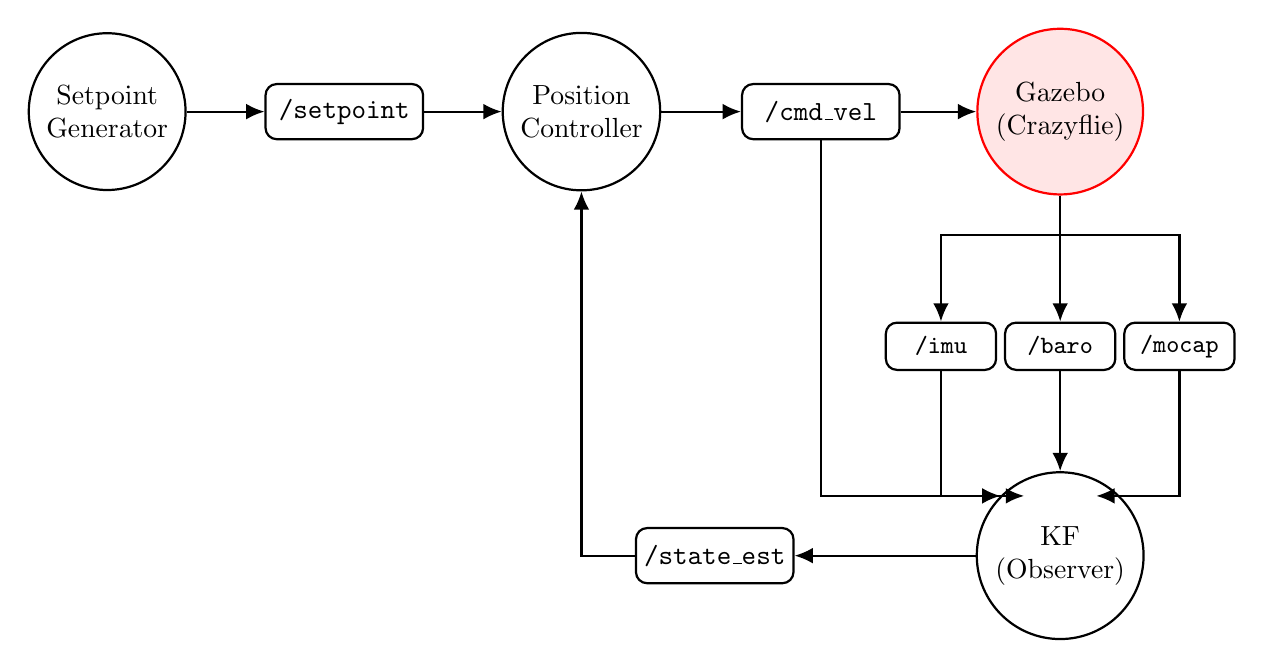
\begin{tikzpicture}[
  node/.style = {circle, draw, thick, minimum size=18mm, align=center},
  gazebo_node/.style = {circle, draw=red, thick, fill=red!10, minimum size=18mm, align=center},
  topic/.style = {draw, thick, rounded corners, minimum height=7mm, minimum width=20mm, align=center, inner sep=2pt},
  sensor_topic/.style = {draw, thick, rounded corners, minimum height=6mm, minimum width=14mm, align=center, inner sep=1pt, font=\small},
  arrow/.style = {thick, -{Latex[width=2mm]}},
  node distance=3.2cm and 2.2cm
]

%--------------------------------------------------
% ROS nodes (circles)
%--------------------------------------------------
\node[node] (setpoint) {Setpoint\\Generator};
\node[node, right=4.0cm of setpoint] (controller) {Position\\Controller};
\node[gazebo_node, right=4.0cm of controller] (gazebo) {Gazebo\\(Crazyflie)};
\node[node, below=3.5cm of gazebo] (observer) {KF\\(Observer)};

%--------------------------------------------------
% Topics (blocks)
%--------------------------------------------------
\node[topic] (t_setpoint) at ($(setpoint)!0.5!(controller)$)
  {\texttt{/setpoint}};

\node[topic] (t_cmd_vel) at ($(controller)!0.5!(gazebo)$)
  {\texttt{/cmd\_vel}};

% Three sensor topics from Gazebo (spread out with smaller boxes)
\node[sensor_topic, below left=1.6cm and 0.8cm of gazebo.south] (t_imu)
  {\texttt{/imu}};

\node[sensor_topic, below=1.6cm of gazebo.south] (t_baro)
  {\texttt{/baro}};

\node[sensor_topic, below right=1.6cm and 0.8cm of gazebo.south] (t_mocap)
  {\texttt{/mocap}};

% feedback topic
\node[topic, left=2.3cm of observer.west] (t_state_est)
  {\texttt{/state\_est}};

%--------------------------------------------------
% Connections
%--------------------------------------------------

% setpoint
\draw[arrow] (setpoint.east) -- (t_setpoint.west);
\draw[arrow] (t_setpoint.east) -- (controller.west);

% cmd_vel
\draw[arrow] (controller.east) -- (t_cmd_vel.west);
\draw[arrow] (t_cmd_vel.east) -- (gazebo.west);

% cmd_vel branch to Observer (south -> northwest)
\draw[arrow]
  (t_cmd_vel.south)
  |- (observer.north west);

% Three sensor topics from Gazebo
\draw[arrow] (gazebo.south) -- ++(0,-0.5) -| (t_imu.north);
\draw[arrow] (gazebo.south) -- (t_baro.north);
\draw[arrow] (gazebo.south) -- ++(0,-0.5) -| (t_mocap.north);

% Sensors to observer (converging)
\draw[arrow] (t_imu.south) |- ($(observer.north west)+(0.3,0)$);
\draw[arrow] (t_baro.south) -- (observer.north);
\draw[arrow] (t_mocap.south) |- ($(observer.north east)+(-0.3,0)$);

% state_est feedback
\draw[arrow] (observer.west) -- (t_state_est.east);
\draw[arrow] (t_state_est.west) -| (controller.south);

\end{tikzpicture}
\end{document}
